\documentclass[a4paper]{report}

\tolerance5000
\usepackage{tgpagella} % Palatino-clone as main font
\linespread{1.05}
\usepackage[a4paper,margin=3cm]{geometry}
\usepackage[utf8]{inputenc}
%\usepackage{times}
\usepackage[english]{babel}
\usepackage{multirow}
\usepackage{amsmath,graphicx}
\usepackage{natbib}
\usepackage{hyperref}
\usepackage{fancyvrb}
\usepackage[textwidth=2.5cm, textsize=small]{todonotes}
\usepackage{listings}
\lstset{% general command to set parameter(s)
  language=Java,
  %keywordstyle=\color{black}\bfseries\underbar, % underlined bold black keywords
  %identifierstyle=,  % nothing happens
  %commentstyle=\color{white}, % white comments
  %numbers=left,
  %numberstyle=\tiny, % the style that is used for the line-numbers
  columns=fixed,
  fontadjust=true,
  basicstyle=\ttfamily,  % typewriter type for strings, add size here if you want
  showstringspaces=false} % no special string spaces

\usepackage{xspace}
\usepackage{tikz}
\usetikzlibrary{arrows.meta}

\newcommand{\vonda}{VOnDA\xspace}

\pgfdeclareimage[width=.99\columnwidth]{vondagui}{VondaGui}
\newcommand{\cmp}[2]{\begin{minipage}[h]{#1}\centering #2\end{minipage}}
% colours in tikz pictures
\definecolor{code}{HTML}{FFE1B6}
\definecolor{midgray}{HTML}{B4B8AB}
\definecolor{darkblue}{HTML}{153243}
\definecolor{ivory}{HTML}{F4F9E9}
\definecolor{lightgray}{HTML}{EEF0EB}
\definecolor{meddarkblue}{HTML}{557C97}

\begin{document}

\title{\vonda\\\Large A Framework for Implementing Reactive Dialogue Agents}

\author{Bernd Kiefer, Anna Welker}
\date{\today}

\maketitle

\tableofcontents

\chapter{Purpose and Goal}

\vonda is a framework to implement the dialogue management functionality in
dialogue systems. Although domain-independent, \vonda is tailored towards
dialogue systems with a focus on social communication, which implies the need
of a long-term memory and high user adaptivity. \vonda's specification and
memory layer relies upon (extended) RDF/OWL, which provides a universal and
uniform representation, and facilitates interoperability with external data
sources. The starting point for designing \vonda was the Information
State-Update approach to dialogue systems, which has a strong resemblance to
the Belief-Desire-Intention approach to Artificial Agents. Thus, it is not
surprising that \vonda can also serve as a base formalism for agent
functionality. A comparison of \vonda to other dialogue management systems and
other related information can also be found in \cite{kieferetal_vonda_2019}.

%\todo[inline]{Mention HFC and ref to appropriate section}
\vonda consists of three parts: A programming language tailored towards the
specification of reactive rules and transparent RDF data store usage, a
compiler that turns source code in this language into Java code, and a run-time
core which supports implementing dialogue management modules using the compiled
rules.

The framework is domain-independent. It was originally designed for multi-modal
human-robot interaction, but there is currently no specific functionality in
the core to either support the multi-modality nor the human-robot
interaction. The architecture (see figure \ref{fig:arch}) of the framework is
open and powerful enough to add these things easily.

%\section{Internal Structure}

\begin{figure}[htb]
\centering
\scriptsize%
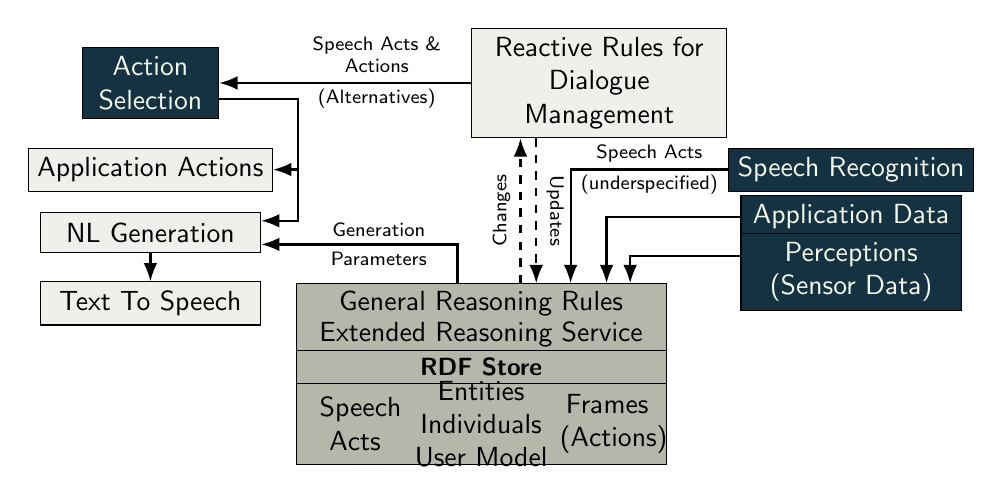
\begin{tikzpicture}[font=\sffamily,
  ampersand replacement=\&,
  box/.style={minimum width=2.8cm, minimum height=.5cm, thin, draw},
  gbox/.style={box, fill=lightgray},
  tbox/.style={box, fill=darkblue, text=ivory},
  ybox/.style={box, fill=lightgray},
  arr/.style={thick, -{Latex}},
  rbox/.style={box, fill=darkblue, text=ivory},
  ]

\path (5.7,3.8) node[gbox, minimum height=1.1cm](rr){\cmp{3cm}{Reactive Rules for\\Dialogue Management}};
\path (0,3.8) node[rbox, minimum width=1.6cm, minimum height=.8cm](as){\cmp{1.5cm}{Action\\Selection}};

\path (8.9,2.7) node[tbox](sr){Speech Recognition};
\path (8.9,2.1) node[tbox](ad){Application Data};
\path (8.9,1.4) node[tbox](per){\cmp{2.2cm}{Perceptions\\(Sensor Data)}};

\path (0,2.7) node[ybox](aa){Application Actions};
\path (0,1.9) node[ybox](nlg){NL Generation};
\path (0,1) node[ybox](tts){Text To Speech};

\path (4.2,0.1) node[box, fill=midgray, minimum width=4.7cm, minimum height=2.3cm](rdf){};
\path (4.2,0.19) node{\small\bf\sffamily RDF Store};
\path (4.2,1) node{General Reasoning Rules};
\path (4.2,0.6) node{Extended Reasoning Service};
\path (2.6,-.53) node{\cmp{.9cm}{Speech\\Acts}};
\path (4.2,-.53) node{\cmp{1.8cm}{Entities\\Individuals\\User Model}};
\path (5.8,-.53) node{\cmp{1.2cm}{Frames\\(Actions)}};

\path (rdf.east) ++(0,-.12) [draw, thin] coordinate(l1) -- (l1 -| rdf.west);
\path (rdf.east) ++(0,.3) [draw, thin] coordinate(l1) -- (l1 -| rdf.west);


\draw[arr] (rr) -- node[above,xshift=4mm,yshift=-4.5mm]{\cmp{2cm}{\scriptsize Speech Acts \& Actions\\[1ex]
    (Alternatives)}} (rr -| as.east);
\path (as.east) ++(0,-.2) [draw, arr] -- ++(1,0) coordinate(here) -|
(here |- aa) coordinate (there) |- (aa);
\path (nlg.east) ++ (0,.15) coordinate (nlg1);
\path (nlg.east) ++ (0,-.15) coordinate (nlg2);
\draw[arr] (there) |- (nlg1);
\path[arr, dashed] (rr.south) ++(-.8,0) coordinate(s1) [draw] -- node[rotate=-90,anchor=south]{\scriptsize Updates} (s1 |- rdf.north);
\path[arr, dashed] (rdf.north) ++(.5,0) coordinate(s2) [draw] -- node[rotate=90,anchor=south]{\scriptsize Changes} (s2 |- rr.south);
\path[arr] (rdf.north) ++(-.3,0) [draw] |- node[below, xshift=-1cm,yshift=4mm]{\cmp{2cm}{\scriptsize Generation\\[.8ex]Parameters}} (nlg2);

\draw[arr] (per.west) ++(0,0.2) -- ++(-1.4,0) coordinate(per1) -- (per1 |- rdf.north);
\draw[arr] (ad.west) -- ++(-1.7,0) coordinate(ad1) -- (ad1 |- rdf.north);
\draw[arr] (sr.west) -- node[above, yshift=-4.4mm]{\cmp{2cm}{\scriptsize Speech
    Acts\\[1ex](underspecified)}} ++(-2,0) coordinate(sr1) -- (sr1 |- rdf.north);

\draw[arr] (nlg) -- (tts);

\end{tikzpicture}
%%% Local Variables:
%%% mode: latex
%%% TeX-master: "vonda"
%%% End:

\caption{\label{fig:arch}Schematic \vonda agent}
\end{figure}

At the base is an RDF store which implements the belief state and takes
incoming sensor and interaction data and stores it as RDF data. The data format
is backed by a data specification in the form of an ontology developed as part
of the dialogue manager, making the data (via the specification) available to
all other components.

The RDF store and reasoner of choice used in \vonda is HFC
\citep{krieger2013efficient}. For further details about the general
functionalities of HFC see chapter \ref{sec:hfc}. Section \ref{sec:example-hfc}
contains an example how HFC is used as database in a \vonda project.

The dialogue manager gets several inputs from various sources, the ones already
used are: input from automatic speech recognition (ASR) or typed natural
language input, user parameters, like name, age, hobbies, etc. but also more
dynamic ones like mood or health data, and also triggers from high-level
planning.

The second major component is the rule processor for the dialogue management
rules. When new data is added, a set of declaratively specified reactive rules
will propose dialogue moves or other actions and send these proposals to the
action selection mechanism. This mechanism selects the ``best'' of the proposed
actions and sends it back. If the proposed action results in dialogue acts,
these are turned into verbal output and gestures with the help of a multimodal
generation component, which retrieves parameters from the RDF database to adapt
the generation to the user's likings, and can also take into account sensor
data such as her or his estimated mood. The rules themselves can use all
available data, the incoming new data, but also the interaction history and
other data stored in the RDF database to make decisions.

The last major component contains the language interpretation module (not
explicitly shown in the picture), which turns spoken or written utterances into
dialogue acts, possibly with an intermediate step that involves a more
elaborate semantic format, and a multimodal generation component, which
converts outgoing dialogue acts into natural language utterances and gestures.

\chapter{A Hands-On Example}
This chapter will walk you through the creation of a simple interaction
manager, which you can either create yourself, or just follow by looking at the
playground system named \texttt{ChatCat}¸ which is placed in the
\texttt{examples} folder. More complex examples are planned to be added soon.

The simplest version of an interaction manager analyses natural language
coming from the user, and generates natural language and gestures for the robot
resp. its virtual replacement, an avatar. Generation is based on incoming
stimuli, like speech or text input, or high-level action requests coming from
some strategic planning component, or any other sensor input, if available.

In this tutorial, we will create a very simple example system that has a
database representation of itself and the user it will interact with. It can
greet the user, ask for his/her name and say goodbye.

\section{Setting up the Basic Data Structures}
\label{sec:example-hfc}

A dialogue system aiming for social interaction does need some kind of memory
representation. Therefore, the first step of building your dialogue manager
with \vonda will be to set up your basic data structures in the form of an OWL
ontology. The RDF database serves two purposes: it contains 1) the data
structure definitions of the data that is used in the dialogue system, like a
\texttt{User} class and the properties that are associated with it, and 2) the
(dynamic) data objects, which are created or extended on-the-fly when the
dialogue system is running. The advantage of using and RDF store for the data
structure specifications lies in its flexibility. Extending or changing them is
easy, which is important since your system will be evolving and becoming more
and more elaborate.

For the specification of dialogue acts, we recommend that you use the dialogue
act hierarchy provided in
\texttt{examples/chatcat/src/main/resources/ontology/dialogue.nt}, which is
based on the ISO standard DIT++ hierarchy, as well as two \texttt{default}
files which are necessary for basic OWL functionality in HFC.

\subsection{Creating N-Triples Files}

%use Protege or another tool of your choice to create OWL/RDF file;
%example here: with Protege
HFC currently loads data only from files in the \texttt{N-Triples} format. The
majority of RDF software packages works with the more common RDF/XML format,
which can be automatically translated with a simple shell script that is
provided with the example (\texttt{examples/chatcat/ntcreate.sh}). This script
uses Raptor \citep{raptor}, which is provided for example in the
\texttt{raptor2-utils} \texttt{.deb} package. This tutorial uses screenshots
from Protégé \citep{Protege}, which we used for the creation of the basic
ontology, but you can just use your favourite RDF/OWL IDE.

First, create a new file that includes an RDF class \texttt{Agent}, and two
subclasses of this class, \texttt{Robot} and \texttt{Human}. After that, create
a (functional) data type predicate \texttt{name} for the class \texttt{Agent}
with the range \texttt{xsd:string}.

\begin{figure}[htb]
  \center
  \begin{minipage}{0.45\textwidth}
    \centering
    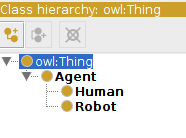
\includegraphics[width=0.6\textwidth]{Images/doc_protege.png}
  \end{minipage}\hfill
  \begin{minipage}{0.45\textwidth}
    \centering
    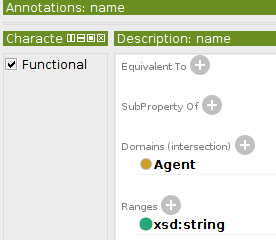
\includegraphics[width=0.6\textwidth]{Images/doc_protege2.png}
  \end{minipage}
\end{figure}

As we do not know the user a priori, we will have the system create an instance
for him/her at run-time. However, we know our robot in advance, so we create an
instance of the class Robot and name it \textit{Robert}, and then convert the
new ontology using Raptor to \texttt{N-Triples} (i.e., with the
\texttt{ntcreate.sh} script). Now, a HFC configuration file (currently in
\texttt{.ini} format) must be created, as described in the next section.

\textbf{Important:} If you are using Prot\'eg\'e, you should save the file in
RDF/XML Syntax; the script will not work properly otherwise.

\subsection{Creating a HFC Configuration File}

%Explain how multiple ontologies can be put together here; explain PersistencyFile, mention what [Namespaces] is about
The ontology files loaded into a HFC instance, and which reasoning rules are
applied, are specified in a configuration file in \texttt{.ini} format. It
also contains various settings for HFC parameters. Figure~\ref{fig:ini} shows
the config file used for the \texttt{chatcat} example. In the following, we
will explain the sections of the config file in detail.

\begin{figure} [htb]
\small%
\begin{verbatim}
[Settings]
#minNoArgs=3
#maxNoArgs=4
#noAtoms=100000
#noTuples=500000
# This file store tuples created or changed during run-time
PersistencyFile=tuples.nt
Encoding=UTF-8

[Namespaces]
# namespaces for XSD, RDF, RDFS, and OWL are already defined
dial = http://www.dfki.de/lt/onto/common/dialogue.owl#
cat = http://www.semanticweb.org/anna/ontologies/2018/3/chatcat#

# instead, you can also load one or more namespace files
#default.ns

[Tuples]
# the axiomatic triples for OWL-Horst w/ EQ reduction
default.eqred.nt

[Tuples]
dialogue.nt
# the name for the base ontology
chatcat.nt

[Rules]
# we need special rules for transaction time (mixture of triples/quadruples)
default.eqred.quads.rdl
\end{verbatim}
\caption{An exemplary HFC \texttt{config.ini} file}
\label{fig:ini}
\end{figure}



\paragraph{[Settings]}

For most applications concerning dialogue management, it is important to
specify a \emph{PersistencyFile} to save the data between two runs of the
system. This file can be put in any location, it will be created automatically
in the specified place. If your application relies on inter-session memory,
you probably don't want it to reside in some temporary directory. All new
information that your dialogue system enters into the database will be
collected here. The persistency file can also be used to find out which tuples
have been created, i.e, for on-line and post-mortem debugging. If you want to
wipe the memory of your system, simply delete this file.

\paragraph{[Namespaces]}

This section contains abbreviations for ontology namespaces. The abbreviation
\texttt{dial} in figure \ref{fig:ini}, allows to refer to
\texttt{<http://www.dfki.de/lt/onto/common/dialogue.owl\#Accept>} using
\texttt{<dial:Accept>} instead, for example in queries to the database. As
you can see, we included a shortcut for our chatcat ontology here.

\paragraph{[Tuples]}

Here all ontology files have to be listed that should be loaded into the
knowledge base on start-up. The persistency file, if you have specified one,
will be loaded automatically. You should also include the file
\texttt{dialogue.nt} which, as previously mentioned, contains the
specifications of the dialogue acts usually used by the \vonda framework.

\paragraph{[Rules]}

This specifies the set of rules that HFC uses for OWL reasoning. Currently, the
file \texttt{default.eqred.quads.rdl} is required for proper operation of
\vonda, since it relies on the so-called \emph{transaction time}
representation, which allows to keep a (possibly) infinite memory, while still
preserving a monotonic RDF store, i.e., only adding and never deleting
tuples. This representation uses quadruples, where the forth element is the
timestamp when the tuple was added to the store. For tuples with infinite
resp. universal validity, the timestamp should be set to zero. For further
information, please refer to the documentation of HFC.

\section{Setting up the Basic Java Classes}

First, the project's abstract (Java) ``agent'' class has to be implemented,
which must be a subclass of \texttt{de.dfki.mlt.rudimant.agent.Agent}, a class
in the run-time library of \vonda. Furthermore, you will need an implementation
of \texttt{de.dfki.mlt.rudimant.agent.CommunicationHub}. To see an example of
what these could contain, take a look in the source folder of \texttt{ChatCat}.

The two most important things here are that there is an active connection to a
database (as an instance of \texttt{RdfProxy}) and that you have an instance of
the beforementioned \vonda \texttt{Agent} wrapper implementation in your
client. Of course this code can not compile until you build your first rule
file, i.e., your \vonda Agent. Then, a \texttt{main} has to create an instance
of your client and is started using the \texttt{startListening()} method.

We recommend to have a look at the classes of the ChatCat system as a base for
your own system and extend it. It comes you with a very simple GUI to enter
text or dialogue acts which you can use to test your first dialogue steps.

\section{Connecting NLU and Generation Components}

%examplary here: srgs for NLU and cplan for generation
Basically, you can connect any NLU and NLG components to your project that are
able to create or, respectively, process dialogue acts of the format that
\vonda provides (cfg. \ref{sec:caret}).

For the sake of simplicity, this example uses SRGS to build a primitive NLU and
cplan\footnote{https://github.com/bkiefer/cplan} to create natural language out of the dialogue acts the agent outputs.

\section{First Interaction Rules}

Now that the basics have been arranged, we are set up for writing our first
dialogue management rules. First we want to react to the user greeting the
system, what we expect to be happening on startup. In the SRGS file
(\small\texttt{src/main/resources/grammars/srgs/chatcat.xml}), we defined that
an utterance of the user like ''Hello'' will be parsed as the dialogue act
\texttt{InitialGreeting}, with the proposition \texttt{Greet}. We now can
define a rule reacting to this utterance:

\begin{lstlisting}
greet_back:
  if (lastDA() <= #InitialGreeting(Greet)) {
    user = new Human;
    if (! saidInSession(#Greeting()) {
      propose("greet_back") {
        emitDA(#ReturnGreeting(Greet));
      }
    }
    lastDAprocessed();
  }
\end{lstlisting}

This will create a new instance of the RDF class \texttt{Human} we defined when
setting up the ontology, storing it in a global variable \texttt{user} that in
our case has been defined in the ChatAgent and will be present during the whole
conversation. The check \texttt{!~saidInSession(\#Greeting)} currently doesn't
seem to make sense, why this is necessary will be obvious when we have
completed the example. This test already shows an important property of the
system: \texttt{Greeting} is the superclass of \texttt{InitialGreeting} and
\texttt{ReturnGreeting} in the DIT++ ontology, and the function will return
\texttt{true}, no matter what type of greeting we gave, since it tests for
\texttt{subsumption}, like the comparison operators \texttt{<=} and \texttt{<}
that work on dialoge act arguments that we use in the next rule example. More
details about how to exploit this functionality will be given in section
\ref{sec:dialogueacts}

After greeting, we want to find out the user's name. We thus define a rule as
follows:

\begin{lstlisting}
ask_for_name:
  if (!user.name && !(myLastDA() <= #WHQuestion(Name))) {
    propose("ask_name") {
      emitDA(#WHQuestion(Name));
    }
    lastDAprocessed();
  }
\end{lstlisting}

And once we got the answer from the user, we can store this knowledge in the
database:

\begin{lstlisting}
remember_name:
  if (lastDA() <= #Inform(Name)) {
    user.name = lastDA().what;
    lastDAprocessed();
  }
\end{lstlisting}

We currently don't have a person detector, so we assume that someone's here
when the system is started. To make sure the conversation starts even if the
user doesn't start with a greeting, we use a \emph{timeout} ot implement a
system greeting after some time.

\begin{lstlisting}
timeout("robot_starts", 4000) {
 start_conversation:
  if (! (receivedInSession(#Greeting(top)) || saidInSession(#Greeting(top)))) {
    propose("robot_greets") {
      tod = Date.timeOfDay();
      emitDA(#InitialGreeting(Greet, when={tod}));
    }
  }
}
\end{lstlisting}
\todo[inline]{Explain the timeOfDay code, and that a Java import and an entry in
  ChatAgent is necessary to obtain compilable code}

These are enough rules to start a conversation, so let's compile and try out
the new dialogue system.

\section{Specifying how to Compile and Run your Project}

Now that we have implemented our first rules, we need to compile them. In the
\texttt{bin} directory of you \vonda installation is a script \texttt{vondac}
that will use you compilation config file to compile your project. The most
convenient way to use it is either to establish a softlink in a directory that
is already in your \texttt{PATH} or to add \vonda's \texttt{bin} directory to
it.

The compile.yml should contain the following parameters:\\

\begin{tabular}{ll}
  \texttt{inputFile} & Relative to the current location, where is the
                       top-level rule file?\\
  \texttt{outputDirectory} & Relative to the current location, where should the compiled classes go?\\
  \texttt{wrapperClass} & The name of your abstract Java Agent, including
                          package prefix\\
  \texttt{ontologyFile} &The path to your ontology \texttt{.ini}, relative to the current location\\
  \texttt{rootPackage} &The topmost package to put the compiled Java classes in\\
  \texttt{failOnError} &If \texttt{true} to exits compilation on any
                         encountered type errors\footnote{Note that although
                         \vonda's type checking is becoming more and more
                         elaborate and reliable, it is by no means complete. In
                         some cases, setting this switch to true might make
                         your project uncompilable although when compiling it
                         ignoring the type errors results in a perfectly sound
                         Java project.}, otherwise continues\\
\end{tabular}\\

Since the compile and the runtime phase of \vonda need different information,
e.g., the run-time phase needs NLU and NLG components, there is a second
\texttt{yaml} file for the run-time phase containing the following
specifications (This is the example from ChatCat):

\begin{verbatim}
ontologyFile:       src/main/resources/ontology/chatcat.ini
NLG:
eng:
mapperProject:      src/main/resources/grammars/cplanner/allrules-mapper
generationProject:  src/main/resources/grammars/cplanner/allrules
NLU:
eng:
class:              de.dfki.chatcat.SrgsParser
grammar:            src/main/resources/grammars/srgs/chatcat.xml
\end{verbatim}

This configuration can be used to start your compiled system by passing it to
the init method of \texttt{Agent}, allowing for easier configuration of these
modules, also in multi-language settings. You can as well put all information
into one \texttt{yaml} file, using it for run time and compile time, since the
irrelevant configuration keys will be ignored.

\subsection{Resolving Name Ambiguities} \label{sec:nsAmbigue}

As you might have noticed whilst looking at chatcat.yml, there is another
parameter used in the compile configuration of our example project:

\begin{verbatim}
nameToURI:
Agent: "<cat:Agent>"

nameToClass:
Date: de.dfki.chatcat.util.Date
\end{verbatim}

When trying to compile without the first two lines, you will find that \vonda
produces the warning \begin{small}'' \texttt{base name Agent can be one of
    <http://www.semanticweb.org/anna/ontologies/2018/3/chatcat\#Agent>,
    <dial:Agent>, please resolve manually.}''
\end{small}.

This is the compiler telling us that when defining the RDF class \texttt{Agent}
in the database step, we actually redefined an existing class. \vonda warns us
about this and urges us to resolve this ambiguity. Thus, we could either rename
our class, or explicitly state which namespace should be accessed whenever the
class \texttt{Agent} is used. \texttt{nameToURI} can be used to do the latter.
You can also use this functionality to remap RDF class names: \vonda will
always map the name on the left to the class URI provided on the right.

The second specification serves to resolve type checks in favour of Java
instead of RDF classes. The fully specified name is currently not used, but
might be used in later versions to generate Java \texttt{import} statements.

% The second specification tells us the \texttt{Date} class' fully specified
% name. This example does not help a lot by itself, but is more relevant if you
% want to use your own support classes providing functionality that is easier
% to implement in Java than in \vonda code. Together with the right field and
% method specifications, this can massively support the type checker. We will
% look into this more closely in section~\ref{sec:support}.

\if0
Natural language dialogue systems are becoming more and more popular, be it as
virtual assistants such as Siri or Cortana, as Chat Bots on websites providing
customer support, or as interface in human-robot interactions in areas ranging
from Industry 4.0 \citep{schwartz2016hybrid} over social human-robot-interaction
\citep{alize2010} to disaster response \citep{kruijff2015tradr}.

A central component of most systems is the \emph{dialogue manager}, which
controls the (possibly multi-modal) reactions based on sensory input and the
current system state. The existing frameworks to implement dialogue management
components roughly fall into two big groups, those that use symbolic
information or automata to specify the dialogue flow (IrisTK
\citep{2012iristk}, RavenClaw \citep{bohus2009ravenclaw}, Visual SceneMaker
\citep{gebhard2012visual}), and those that mostly use statistical methods
(PyDial \cite{ultes2017pydial}, Alex \citep{jurvcivcek2014alex}). Somewhat in
between these is OpenDial \citep{lison2015developing}, which builds on
probabilistic rules and a Bayesian Network.

When building dialogue components for robotic systems or in-car assistants, the system
needs to take into account \emph{various} system inputs, first and foremost the
user utterances, but also other sensoric input that may influence the dialogue,
such as information from computer vision, gaze detection, or even body and
environment sensors for cognitive load estimation.

The integration and handling of the different sources such that all data is
easily accessible to the dialogue management is by no means trivial. Most
frameworks use plug-ins that directly interface to the dialogue core. The
multi-modal dialogue platform SiAM-dp \citep{nesselrath2014siam}
addresses this in a more fundamental way using a modeling approach that allows
to share variables or objects between different modules.

In the application domain of social robotic assistants, it is vital to be able
to maintain a relationship with the user over a longer time period. This requires a long-term
memory which can be used in the dialogue system to exhibit familiarity with the
user in various aspects, like personal preferences, but also common knowledge
about past conversations or events, ranging over multiple sessions.

In the following, we will describe \vonda, an open-source framework to
implement dialogue strategies. It follows the information state/update
tradition \citep{traum2003information}
%DR Traum, S Larsson. The information state approach to dialogue management. In: Current and new directions in discourse and dialogue, 2003, pp.  325-353. Kluwer.
combining a rule-based approach with statistical selection, although in a
different way than OpenDial. \vonda specifically targets the following design
goals to support the system requirements described before:

\begin{itemize}
  \addtolength{\itemsep}{-.6\itemsep}
\item Flexible and uniform specification of dialogue semantics, knowledge and
  data structures
\item Scalable, efficient, and easily accessible storage of interaction history
  and other data, resulting in a large information state
\item Readable and compact rule specifications, facilitating access to the
  underlying RDF database, with the full power of a programming language
\item Transparent access to Java classes for simple integration with the host
  system
\end{itemize}
\fi

%%% Local Variables:
%%% mode: latex
%%% TeX-master: "userguide"
%%% End:


\chapter{Structured Overview}
\section{Rudimant-Kompiler und Laufzeitsystem}

Der Rudimant-Kompiler übersetzt Regeldateien mit Extension \texttt{.rudi} in
Java-Dateien. Dazu braucht er eine Ontologie, in der die RDF Klassen und
Prädikate, die im \texttt{.rudi}-Code verwandt werden, spezifiziert sind.

Im Fall des POC liegen die Quelldateien in \texttt{src/main/rudi} und die
dazugehörende Ontologie in \texttt{src/main/resources/ontology}. Damit HFC
die Ontologie benutzen kann, muss sie im ntriples-Format vorliegen. Die
derzeitige Ontologie wird mit Protégé erstellt und aus dem OWL-XML Format
mit Hilfe des \texttt{rapper}-Tools in eine \texttt{.nt} ntriples Datei
übersetzt. \texttt{rapper} ist Teil des Ubuntu-Package \texttt{raptor2-utils},
das Script \texttt{ntcreate} im \texttt{poc} Verzeichnis updated alle nicht
aktuellen \texttt{.nt} Files aus den \texttt{.owl} Versionen.

Weitere settings, die für die Kompilation wichtig sind, finden sich in der
Datei \texttt{herbea.yml}, die von \texttt{compile} Skript benutzt wird. Auch
hier sind alle relativen Pfade relativ zum Verzeichnis, in dem die
\texttt{.yml} Datei liegt.

Für standalone Mockup-Tests kann der POC auch isoliert mit dem \texttt{run.sh}
script gestartet werden, die ``Sensordaten'' werden dann nach und nach in
der main-Methode eingespielt.

Der folgende Text ist leider unvollständig und muss noch ergänzt werden. Für
die meisten Konstrukte gibt es einige Beispiele in den \texttt{rudi}
Quelldateien.

\subsection{Rudimant Regeln}

%{\Huge TODO: testen, ob alle Beispiele so funktionieren, wie sie sollen !!!!!!}

\subsubsection{''Globale'' Funktionen und Variablen}

Für Funktionen, die nicht oder nur umständlich in rudi-Code implementiert werden können, sollte der Nutzer eine Javaklasse MyAgent von der abstrakten Klasse Agent ableiten. Funktionen und Variablen, die in dieser Klasse deklariert wurden und später im rudi-Code benutzt werden sollen, müssen mit vollständiger Typangabe in einer Datei MyAgent.rudi registriert werden, sodass die Typinferenz von rudimant sie korrekt berücksichtigen kann (zur Syntax siehe \ref{rudimant-Typinferenz}).\\
Die Klasse MyAgent mitsamt Packagenamen muss in der config.yml Datei eines Projektes unter dem Eintrag ''wrapperClass'' spezifiziert werden, um im Compile-Schritt einen Effekt zu zeigen. Rudimant nutzt die Klasse MyAgent dann als Superklasse der im Compile-Schritt angegebenen Datei im rudi-Format und verlinkt Funktionsaufrufe und Variablennutzungen in allen untergeordneten rudi-Dateien auf diese, sodass korrekte Aufrufe im resultierenden Java-Code gewährleistet sind.

\subsubsection{RDF Zugriff, funktionale vs. relationale Prädikate
  \texttt{+=}, \texttt{-=}}

\begin{minipage}{0.4\textwidth}
\begin{verbatim}
Child c;
String name = c.name;
c.name = "new name";
\end{verbatim}
\end{minipage}
\begin{minipage}{0.6\textwidth}
\begin{verbatim}
String name = (String)c.getValue("<upper:name>");
c.setValue("<upper:name>", "new name");
\end{verbatim}
\end{minipage}
\newline
Durch die Verbindung zu hfc während des Compile-Vorganges hat rudimant vollen Zugriff auf die Datenbank und kann nicht nur Rdf-Objekte anhand ihrer Typen erkennen, sondern auch erkennen, wann ein Feldzugriff auf ein Rdf-Objekt erfolgt und ihn in solchen Fällen in einen Zugriff auf die Datenbank umwandeln. Dies ist sowohl für Zugriffe auf Properties als auch für Änderungen ihres Inhalts möglich und lässt sich, sofern dies in der verwendeten Ontologie möglich ist, beliebig oft hintereinander ausführen.\\

TODO: funktional vs relational?

Die beiden Operatoren \texttt{+=} und \texttt{-=} sind in rudimant überladen. Sie können sowohl wie in Java zum Rechnen mit Integer, float und double verwendet werden, als auch im Zusammenspiel mit Sets und Listen. $ a += b $ wird hierbei in $ a.add(b) $ umgewandelt, $ a-= b $ resultiert in $ a.remove(b) $.
  
\subsubsection{Regeln und Labels}

\begin{verbatim}
introduction:
  if (introduction){
    if (user.unknown){
      ask_for_name:
        if (talkative) {
          askForName();
        }
    } else {
      greetUser();
    }
  }
\end{verbatim}

Das Kernstück von rudimant sind die Dialogregeln. Eine Regel beginnt mit ihrem Namen, einem möglichst aussagekräftigen Label, gefolgt von einem Doppelpunkt. Anschließend folgt ein if-statement. Die Clause des Statements drückt die Bedingung aus, unter der die Regel ausgeführt werden soll, im Body steht der auszuführende Code.\\
Aussagekräftige Labels sind zum Debugging wichtig. Der generierte Code kann zur Laufzeit debuggt werden, indem man in Agent den Flag ... setzt. Der Output des Loggers wird dann das Label jeder Regel, die evaluiert wird, zusammen mit der Auswertung der Bedingung angeben.\\
% Bsp debugging-output
Regeln können beliebig tief geschachtelt werden, d.h., jede Regel kann wiederum Subregeln in ihrem Body haben.

%\subsubsection{Propose}

\subsubsection{Struktur einer Datei im rudi-Format}

Anders als Java stellt rudimant nicht den Anspruch, dass die Einträge in einer Datei in irgendeine Form von übergeordneter Struktur gefasst werden. Die Regeln können ebenso wie Funktionsdeklarationen direkt in die Datei geschrieben werden. Dasselbe gilt für jede Art valider (Java-) Statements, wie etwa Zuweisungen, for-Schleifen usw.. Rudimant wird bei der Kompilation eine Java-Klasse erstellen, in die es die Funktionen sowie die Regeln, zu Funktionen transformiert, einträgt. Alle weiteren Statements werden in der korrekten Reihenfolge in die erzeugte Methode process() verschoben, wobei generierte Aufrufe an die Regelfunktionen zwischen ihnen gewährleisten, dass die Regeln und Statements in der Reihenfolge ausgeführt werden, die im rudi-Code spezifiziert war. Dies ermöglicht also, nicht in Regeln gefasste Abbruchbedingungen einzubauen, unter denen die Ausführung der ganzen Datei - und möglicher importierter Dateien - sofort beendet werden soll.\\
Auf diese Art deklarierte Variablen werden als Klassenvariablen angelegt.

\subsubsection{Dialogakte und Hütchen} \ {\Large\verb|^|}

\begin{verbatim}
emitDA(#Inform(Answer, what=^solution));
\end{verbatim}

\subsubsection{Typinferenz} \label{rudimant-Typinferenz}

Rudimant erlaubt statische Typzuweisungen sowie Casting, beides ist jedoch nicht zwingend notwendig.\\
Ist beispielsweise der Typ der rechten Seite einer Variablendeklaration mit Zuweisung bekannt oder inferierbar, so ist es nicht notwendig, den Typ der Variablen explizit anzugeben.\\
Als zeitsparendes Feature bietet rudimant insbesondere das automatische Vervollständingen von bool'schen Ausdrücken in den Clauses von if, while und for an. Da in diesem Fall bekannt ist, dass das Ergebnis boolean sein muss, ergänzt rudimant automatisch den Test auf die Existenz eines Objektes in der Clause, sollte dieses nicht Typ boolean sein. Bei Feldzugriffen testet es für jeden Teilzugriff, dass das erhaltene Objekt nicht null ist, um einer NullPointerException zur Laufzeit des generierten Codes vorzubeugen.

\subsubsection{Überladene Vergleichsoperatoren und Tests}

\begin{minipage}{0.4\textwidth}
\begin{verbatim}
if (speechAct <= #Question){
  ...
}
\end{verbatim}
\end{minipage}
\begin{minipage}{0.6\textwidth}
\begin{verbatim}
if (isSmallerEqual(speechAct, new DialogueAct("Question")) {
  ...
}
\end{verbatim}
\end{minipage}
\newline


\begin{minipage}{0.4\textwidth}
\begin{verbatim}
if (! c.user.personality.nonchalance){
  ...
}
\end{verbatim}
\end{minipage}
\begin{minipage}{0.6\textwidth}
\begin{verbatim}
if (!((((c != null) && (c.user != null))
      && (c.user.personality != null))
      && (c.user.personality.nonchalance != null))) {
  ...
}
\end{verbatim}
\end{minipage}

\subsubsection{Funktionale Konstrukte (lambda)}
\begin{verbatim}
boolean contains(Collection coll, Predicate pred);
boolean all(Collection coll, Predicate pred);
List<Object> filter(Collection coll, Predicate pred);
List<Object> sort(Collection coll, Comparator c);
\end{verbatim}

\subsubsection{\texttt{import}}

%\begin{itemize}
%\item ``Globale'' Funktionen und Variablen
%\item RDF Zugriff, funktionale vs. relationale Prädikate
%  \texttt{+=}, \texttt{-=}
%\item Regeln und Labels
%%\item \texttt{propose}
%\item Dialogakte und\ {\Large\verb|^|}
%\item Typinferenz
%\item Überladene Vergleichsoperatoren und Tests
%\item Funktionale Konstrukte (lambda)
%\item \texttt{import}
%\end{itemize}

\subsection{Struktur des POC Rudimant-Projekts}

TODO: Siehe Bild für Softprak, Beschreibung von HerbeaAgent.rudi
vs. HerbeaAgent.java und Rolle von HerbeaClient

Die Basisklassen von Herbea sind \texttt{HerbeaClient}, der die Kommunikation
mit der Außenwelt herstellt, und \texttt{HerbeaAgent}, der Java-Funktionalität
zur Verfügung stellt, die sich nicht ohne weiteres in \texttt{rudi} Dateien
implementieren lässt (komplexe Queries an die Datenbank, etc.).

Zu \texttt{HerbeaAgent.java} gehört noch eine Datei \texttt{HerbeaAgent.rudi},
die sozusagen das Interface beschreibt, auf das der \texttt{rudi} Quellcode
zugreifen kann. Hier können auch statt der generischen Klasse \texttt{Rdf} die
Klassen aus der Ontologie spezifiziert werden, wenn diese genauer angegeben
werden können. Das hilft dem Kompiler bei der Typinferenz und dem richtigen
Zugriff mit RDF-Prädikaten.

\subsection{Default-Funktionalität im Laufzeitsystem}
Alles was in \texttt{Agent} bereitgestellt wird. Die aktuelle Liste der
bereitgestellten Funktionen finden sich in \texttt{rudimant} unter
\texttt{src/main/resources/Agent.rudi}.

\begin{itemize}
\item timeouts
\begin{verbatim}
void newTimeout(String name, int millis);
boolean isTimedOut(String name);
void removeTimeout(String name);
boolean hasActiveTimeout(String name);
\end{verbatim}
\item Senden von Dialogakten an die Generierung
\begin{verbatim}
DialogueAct emitDA(int delay, DialogueAct da);
DialogueAct emitDA(DialogueAct da);
\end{verbatim}
\item Zugriff auf DialogAkte aus der Session
\begin{verbatim}
// my last outgoing resp. the last incoming dialogue act
DialogueAct myLastDA();
DialogueAct lastDA();

// did i say something like ta in this session (subsumption)? If so, how many
// utterances back was it? (otherwise, -1 is returned)
int saidInSession(DialogueAct da);
// like saidInSession, only for incoming dialogue acts
int receivedInSession(DialogueAct da);

boolean waitingForResponse();
void lastDAprocessed();
\end{verbatim}
\end{itemize}

%%% Local Variables:
%%% mode: latex
%%% TeX-master: "master"
%%% End:

\newpage
\section{Debugger/GUI}
\label{sec:debugger}

\vonda comes with a GUI \citep{rudibuggerThesis} that helps navigating, compiling and editing the source files belonging to a project. It can also be attached to your \vonda project at runtime to support debugging by logging the evaluation of rule conditions.

\begin{figure}[thb]

  \centering
  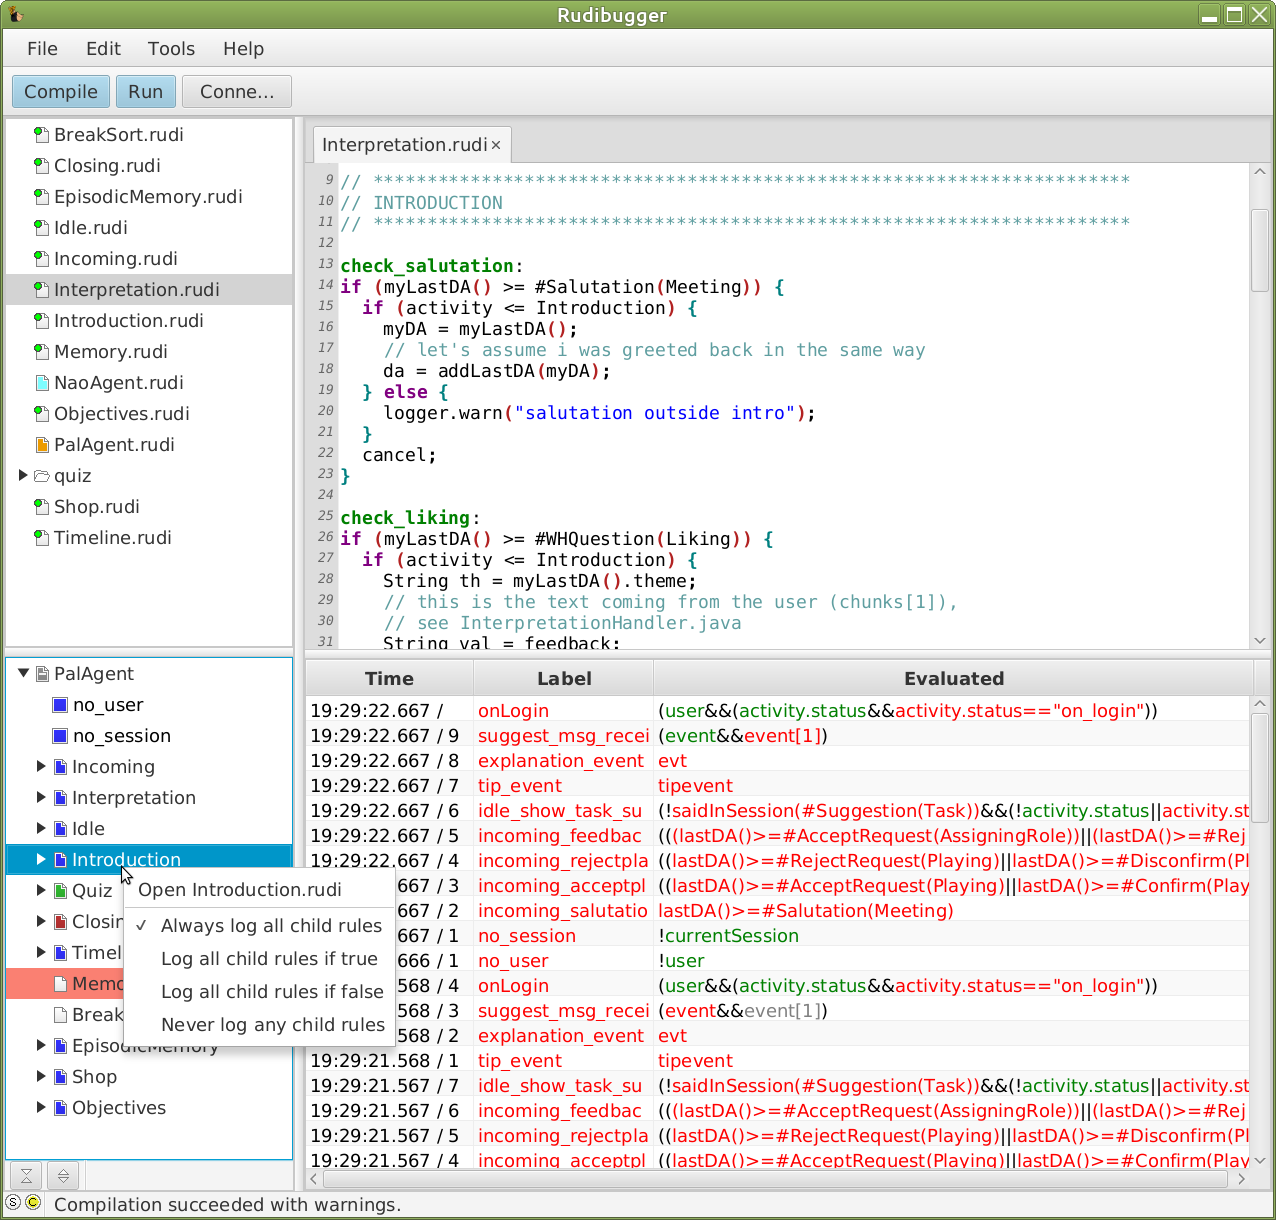
\includegraphics[width=.8\textwidth]{VondaGui.png}
  \caption{The \vonda GUI window}
  \label{vondagui}
\end{figure}

For further details, please take a look into rudibuggers own documentation. The project can be found on \url{https://github.com/yoshegg/rudibugger}.
\newpage
\section{The RDF Database HFC} \label{sec:hfc}

\vonda follows the information state/update paradigm. The information state is
realized by an RDF store and reasoner with special capabilities
(HFC \cite{krieger2013efficient}), namely the
possibility to directly use $n$-tuples instead of triples. This allows to
attach temporal information to every data chunk \cite{Krieger:FOIS2012,
  krieger2014detailed}. In this way, the RDF store can represent \emph{dynamic
  objects}, using either \emph{transaction time} or \emph{valid time}
attachments, and as a side effect obtain a complete history of all changes.
HFC is very efficient in terms of processing speed and memory footprint, and
has recently been extended with stream reasoning facilities. \vonda can use HFC
\todo{AW: Just asking: How long can we still talk of ''recently extended''?}
either directly as a library or as a remote server, also allowing for more
than one instance if needed (for this feature see section \ref{sec:2ndHfc}).

The following is the syntax of HFC queries (EBNF):
\begin{table}[htbp]
  \centering\small
\begin{verbatim}
<query>     ::= <select> <where> [<filter>] [<aggregate>] | ASK <groundtuple>
<select>    ::= {"SELECT" | "SELECTALL"} ["DISTINCT"] {"*" | <var>^+}
<var>       ::= "?"{a-zA-Z0-9}^+ | "?_"
<nwchar>    ::= any NON-whitespace character
<where>     ::= "WHERE" <tuple> {"&" <tuple>}^*
<tuple>     ::= <literal>^+
<gtuple>    ::= <constant>^+
<literal>   ::= <var> | <constant>
<constant>  ::= <uri> | <atom>
<uri>       ::= "<" <nwchar>^+ ">"
<atom>      ::= "\""  <char>^* "\"" [ "@" <langtag> | "^^" <xsdtype> ]
<char>      ::= any character, incl. whitespaces, numbers, even '\"'
<langtag>   ::= "de" | "en" | ...
<xsdtype>   ::= "<xsd:int>" | "<xsd:long>" | "<xsd:float>" | "<xsd:double>" |
                "<xsd:dateTime>" | "<xsd:string>" | "<xsd:boolean>" | "<xsd:date>" |
                "<xsd:gYear>" | "<xsd:gMonthDay>" | "<xsd:gDay>" | "<xsd:gMonth>" |
                "<xsd:gYearMonth>" | "<xsd:duration>" | "<xsd:anyURI>" | ...
<filter>    ::= "FILTER" <constr> {"&" <constr>}^*
<constr>    ::= <ineq> | <predcall>
<ineq>      ::= <var> "!=" <literal>
<predcall>  ::= <predicate> <literal>^*
<predicate> ::= <nwchar>^+
<aggregate> ::= "AGGREGATE" <funcall> {"&" <funcall>}^*
<funcall>   ::= <var>^+ "=" <function> <literal>^*
<function>  ::= <nwchar>^+
\end{verbatim}
  \caption{BNF of the database query language}
  \label{tab:hfcquerybnf}
\end{table}

%\paragraph{Notes}

The reserved symbols \texttt{ASK}, \texttt{SELECT}, \texttt{SELECTALL},
\texttt{DISTINCT}, \texttt{WHERE}, \texttt{FILTER} and \texttt{AGGREGATE}
do \emph{not} need to be written in uppercase, but neither \texttt{filter} predicates nor \texttt{aggregate} functions should be named like reserved symbols.

\emph{don't-care} variables should be marked \emph{explicitely} by using
\verb|?_|, particularly if \texttt{SELECT} is used with \verb|*| as in:
\begin{verbatim}
     SELECT DISTINCT * WHERE ?s <rdf:type> ?_
     SELECT * WHERE ?s <rdf:type> ?o ?_
\end{verbatim}
To change the object position without projecting it you can use \emph{don't-care} variables:
\todo{AW: I do have an idea of how to write hfc queries of the simplicity that is sufficient for most DM stuff, and I have no understanding of what this means... Explain?}
\begin{verbatim}
     SELECT ?s WHERE ?s <rdf:type> ?o ?_ FILTER ?o != <foo-class>
\end{verbatim}

Aggregates in HFC take whole tables or parts of them and calculate a result based on their entities. As the type of aggregates and filter functions cannot be overloaded, there are multiple similar functions for different types, e.g. F for \texttt{float}, L for \texttt{long}, D for \texttt{double}, I
for \texttt{int}, and S for \texttt{String}.

\begin{table}[htbp]
  \centering
 \begin{tabular}{lll}
   CountDistinct&  FSum&             LMax\\
   Count&          FMean&            LMean\\
   DMean&          LGetFirst2&       LMin\\
   DSum&           LGetLatest2&      LSum\\
   DTMax&          LGetLatest&       LGetLatestValues\\
   DTMin&          LGetTimestamped2& Identity     \\
 \end{tabular}
  \caption{Available aggregates}
  \label{tab:hfcaggregates}
\end{table}

Apart from \verb|==| and \verb|!=|, functional operators can be used in \texttt{filter} expressions as well. As for aggregates, there are multiple versions of the same function for different data types.

\begin{table}[htbp]
  \centering\small
\begin{tabular}{llll}
CardinalityNotEqual &        FNotEqual &               IntStringToBoolean &      LMin \\
Concatenate &                FProduct &                IProduct &                LNotEqual \\
DTIntersectionNotEmpty &     FQuotient &               IQuotient &               LProduct \\
DTLessEqual &                FSum &                    IsAtom &                  LQuotient \\
DTLess &                     GetDateTime &             IsBlankNode &             LSum \\
DTMax2 &                     GetLongTime &             IsNotSubtypeOf &          LValidInBetween\\
DTMin2 &                     HasLanguageTag &          ISum &                    MakeBlankNode \\
EquivalentClassAction &      IDecrement &              IsUri &                   MakeUri \\
EquivalentClassTest &        IDifference &             LDecrement &              NoSubClassOf \\
EquivalentPropertyAction &   IEqual &                  LDifference &             NoValue \\
EquivalentPropertyTest &     IGreaterEqual &           LEqual &                  PrintContent \\
FDecrement &                 IGreater &                LGreaterEqual &           PrintFalse \\
FDifference &                IIncrement &              LGreater &                PrintSize \\
FEqual &                     IIntersectionNotEmpty &   LIncrement &              PrintTrue \\
FGreaterEqual &              ILessEqual &              LIntersectionNotEmpty &   SameAsAction \\
FGreater &                   ILess &                   LIsValid &                SameAsTest \\
FIncrement &                 IMax2 &                   LLessEqual &              SContains.java\\
FLessEqual &                 IMax &                    LLess &                   UDTLess \\
FLess &                      IMin2 &                   LMax2 \\
FMax &                       IMin &                    LMax \\
FMin &                       INotEqual &               LMin2 \\
\end{tabular}
\caption{Available filter functions}
  \label{tab:hfcfunctions}
\end{table}

\subsection{Usage of HFC in \vonda} \label{sec:hfc_usage}

The RDF store contains the dynamic and the terminological knowledge:
specifications for the data objects and their properties, as well as a
hierarchy of  dialogue acts,  semantic frames and their arguments. These
specifications are also used by the compiler to infer the types for property
values (see sections \ref{sec:typeinference} and \ref{sec:rdfaccesses}), and form a declarative API to
connect new components, e.g., for sensor or application data.

The ontology contains the definitions of dialogue acts, semantic frames, class
and property specifications for the data objects of the application, and other
assertional knowledge, such as specifications for ``forgetting'', which could
be modeled in an orthogonal class hierarchy, and supported by custom deletion
rules in the reasoner.

For queries which are too complex to be handled the \vonda way, or if you want to do reasoning which for efficiency reasons should be handled by HFC rather than Java (e.g., if you are filtering for specific property values in a pool of many instances of the same class), there also is a direct communication port to HFC.

\begin{lstlisting} [language=Java]
List<String> uris = new ArrayList<>();
// the ancestor is that hyponym which has the shortest path to syn
String ancestors = "select ?s  where ?s <wn20schema:hyponym> {} ?_ ";
QueryResult qr = proxy.selectQuery(ancestors, syn);
uris = RdfProxy.getValues(qr);
\end{lstlisting}

The above code, for example, retrieves all hyponyms of a given synset \texttt{syn}.

Currently, it is recommended to place such code in Java methods that you can then use in your \vonda code to indirectly perform the queries. In the future, functionality will be added to support facilitated query construction directly in \vonda code.


% implementation patterns and caveats
\chapter{Building \vonda Agents}
\section{Implementation Patterns and Caveats}

\subsection{Proper Usage of \texttt{lastDAprocessed} and \texttt{emitDA}}

\todo{Actually, shouldn't we already explain lastDAprocessed somewhere else?}
\texttt{lastDAprocessed} is a built-in method that helps you clean up after a dialogue act has been dealt with. You usually want to call it in your \texttt{propose} block, because when the block is executed that means that the dialogue act has been processed. The method's effect is to set an internal timestamp of the moment it has been called, which affects the return value of \texttt{lastDA}: \texttt{lastDA} will only return a dialogue act if it has been sent after the the time of \texttt{lastDAprocessed} timestamp.

Be aware this also means that if the statement you execute in your \texttt{propose} block is \texttt{lastDAprocessed();}, all following calls to \texttt{lastDA()} will evaluate to an empty dialogue act. Thus, using expressions like \texttt{theme=lastDA().theme} in an \texttt{emitDA} are strongly discouraged, because they will fail if the \texttt{emitDA} is used after calling the cleanup method. There is, however, good reason to not move the \texttt{lastDAprocessed} to the very end of your proposal, as proposals are executed in a separate thread and your 
\vonda rules are executed in parallel. This might, in rare cases where your proposal code takes more time to process (for one possible reason, see \ref{emitDA}), lead to your system generating and executing new proposals based on the ''old'' dialogue act, thus responding more than once to one input.

\subsection{A Few Words About \texttt{emitDA} and \texttt{createBehaviour}} \label{emitDA}
\newpage
% and maybe tips and tricks?
\chapter{\vonda Syntax Overview}
\input{AllYouCanDo.rudi}

\bibliography{vonda}
\bibliographystyle{plainnat}

\end{document}
